The aim of this chapter is to test and analyze projects from git by using the developed module for RefactorErl. Git commit logs hold all the change history. This is an excellent source to observe trends and patterns about projects. All projects selected for the experiment are written in Erlang and have more than 40 commits.

\section{Iron}

This project is functional Erlang Toolkit. Iron is released under the MIT license. It can do the foolowing:
\begin{itemize}
	\item Count with coerce equality, count with a custom predicate.
	\item Find with coerce equality, find with a custom predicate.
\end{itemize}

This project has just only one source code file with 68 commits. The link to the repository is \url{https://github.com/elementerl/iron}.

We can see that with the version number increase the line of code number and char of code number also grow on Figure \ref{fig:loc_iron} and in Figure \ref{fig:char_iron}.

\begin{figure}[h]
	\centering
	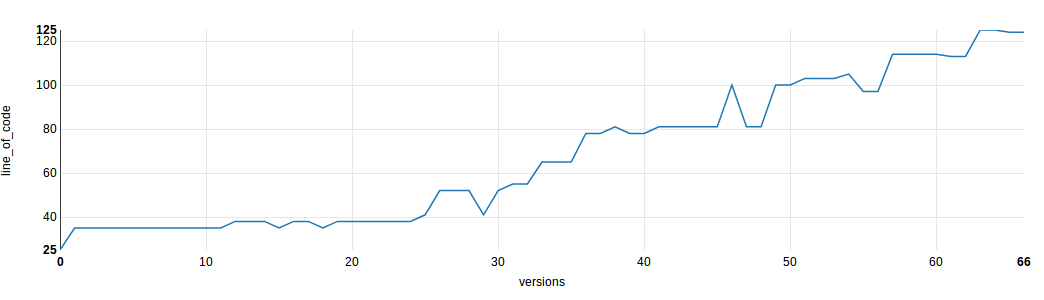
\includegraphics[height=45mm]{figures/loc_iron.png}
	\caption{Effective Line of code for fe.erl file.}
	\label{fig:loc_iron}
\end{figure}

\begin{figure}[h]
	\centering
	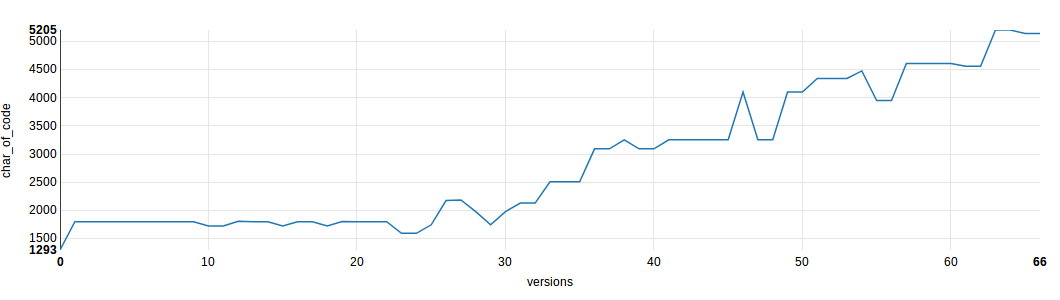
\includegraphics[height=45mm]{figures/char_iron.png}
	\caption{Char of code for fe.erl file.}
	\label{fig:char_iron}
\end{figure}

As shown in Figure \ref{fig:otp_iron} developer started to use otp library after 45th version. 

\begin{figure}[h]
	\centering
	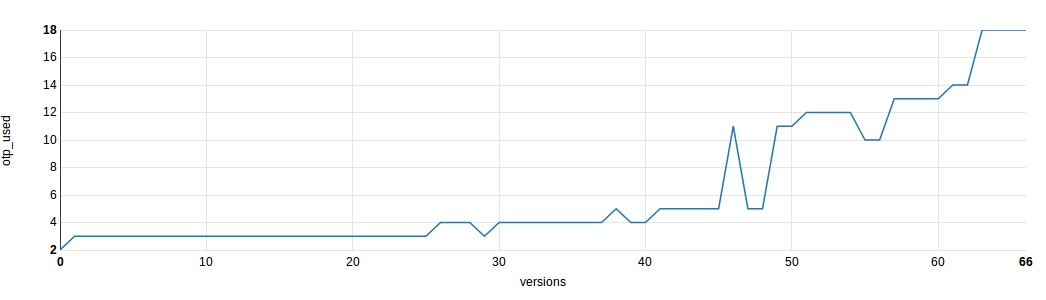
\includegraphics[height=45mm]{figures/otp_iron.png}
	\caption{Otp used for fe.erl file.}
	\label{fig:otp_iron}
\end{figure}

The Figure \ref{fig:mcCabe_iron} shows an overview of the evolution of the overall McCabe cyclomatic complexity. We can observe that the complexity keeps increasing.

There was a spike in 45th version, because some functions were called to an other module, however author removed changes in 46th version. There was also an insignificant drop in complexity in 28th version and a little increase in 29th version. The  complexity decreases  when  the  extracted  piece  of code occurred more than one time and the complexity of the function is more than one~\cite{mcCabe}. 

In Figure \ref{fig:max_depth_of_cases_iron} we can see that the metric \textbf{max\_depth\_of\_cases} is 1, but before it was 0, therefore developer stopped using case inside another case for this version of the software. We can find the same trend on plot with \textbf{mcCabe} metric where it appears as decreasing of the program complexity.  

\begin{figure}[h]
	\centering
	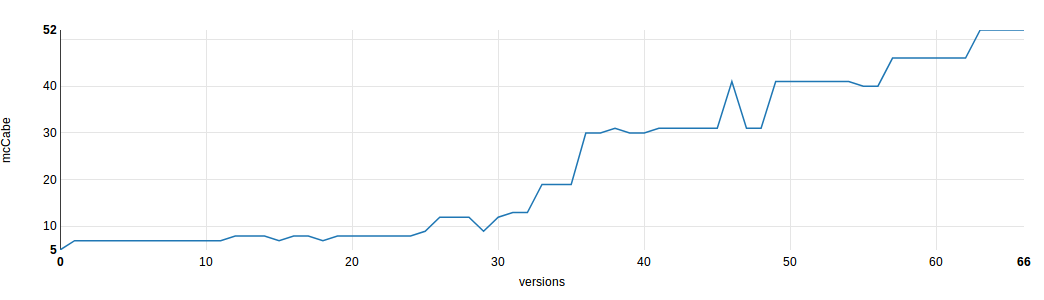
\includegraphics[height=45mm]{figures/mcCabe_iron.png}
	\caption{McCabe cyclomatic complexity metric for fe.erl file.}
	\label{fig:mcCabe_iron}
\end{figure}

\begin{figure}[h]
	\centering
	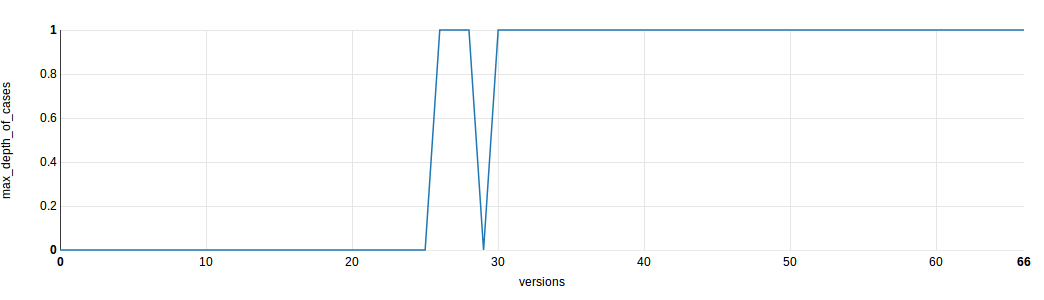
\includegraphics[height=45mm]{figures/max_depth_of_cases_iron.png}
	\caption{Max depth of cases for fe.erl file.}
	\label{fig:max_depth_of_cases_iron}
\end{figure}

The average length of the line was not stabilized until 35th version with gradually decreasing from 50 symbols to 38 symbols in Figure \ref{fig:average_length_of_line_iron}.

\begin{figure}[h]
	\centering
	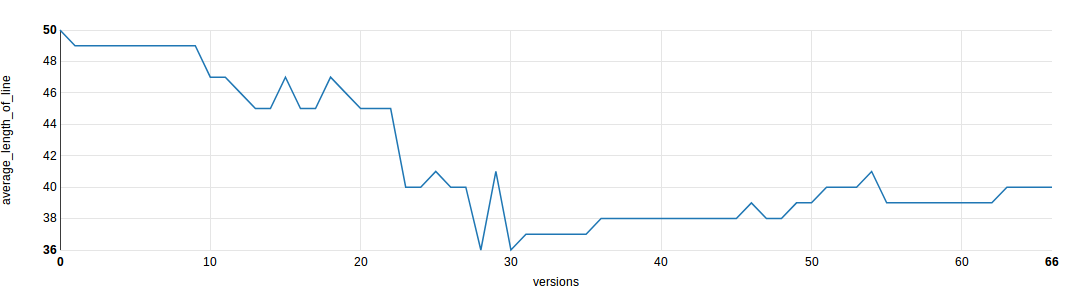
\includegraphics[height=45mm]{figures/average_length_of_line_iron.png}
	\caption{Average length of line for fe.erl file.}
	\label{fig:average_length_of_line_iron}
\end{figure}

As we can see in Figure \ref{fig:number_of_macros_iron} and Figure \ref{fig:number_of_records_iron} there are not defined macroses and records in the whole iron project.

\begin{figure}[h]
	\centering
	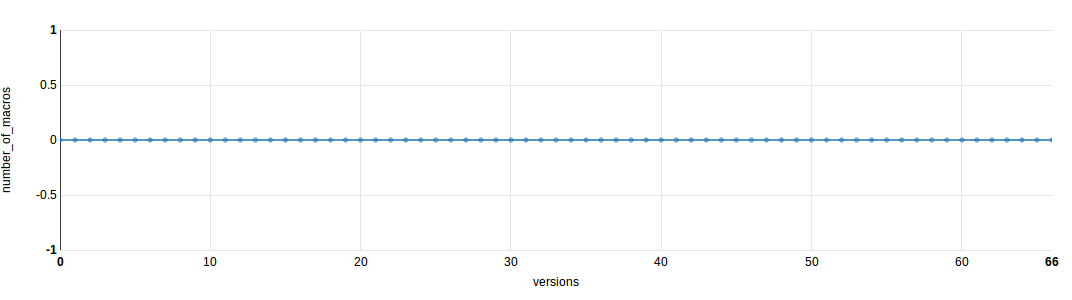
\includegraphics[height=45mm]{figures/number_of_macros_iron.png}
	\caption{Number of macros for fe.erl file.}
	\label{fig:number_of_macros_iron}
\end{figure}

\begin{figure}[h]
	\centering
	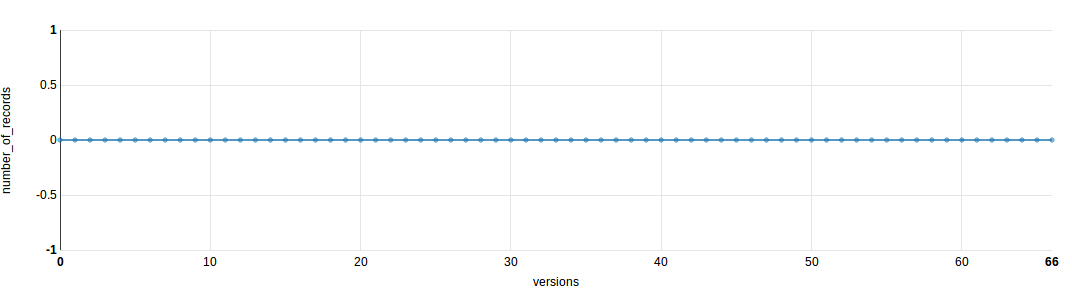
\includegraphics[height=45mm]{figures/number_of_records_iron.png}
	\caption{Number of records for fe.erl file.}
	\label{fig:number_of_records_iron}
\end{figure}
%%____________________________________________________________________-

\section{Erlang chat }

This project is multi-user chat written in Erlang. It has nine source code files and 45 commits. The link to the repository is \url{https://github.com/bildeyko/erlangChat}

For this project, we analyzed the module \textbf{websocket\_handler.erl}. This module consists of 6 functions.

We can see an increasing number of lines of code in Figure \ref{fig:loc_chat} and an increasing number of characters in a program text in Figure \ref{fig:char_of_code_chat}.

\begin{figure}[h]
	\centering
	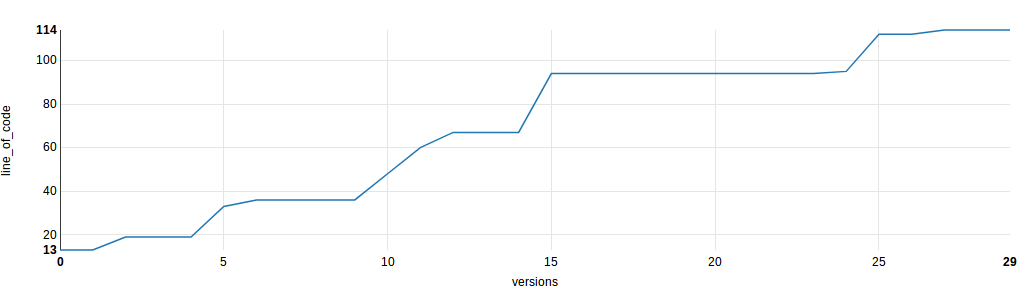
\includegraphics[height=45mm]{figures/loc_chat.png}
	\caption{Effective Line of code for module websocket\_handler.erl.}
	\label{fig:loc_chat}
\end{figure}

\begin{figure}[h]
	\centering
	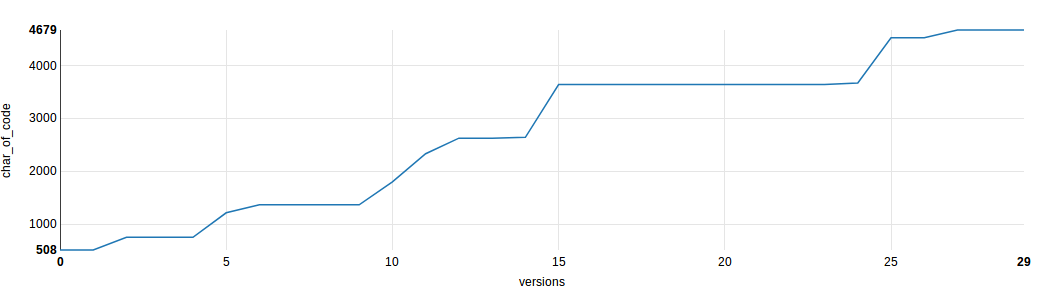
\includegraphics[height=45mm]{figures/char_of_code_chat.png}
	\caption{Characters of the code for module websocket\_handler.erl.}
	\label{fig:char_of_code_chat}
\end{figure}

In Figure \ref{fig:chat} we can see that the author started using message passing from the 9th version of his software.

\begin{figure}[h]
	\centering
	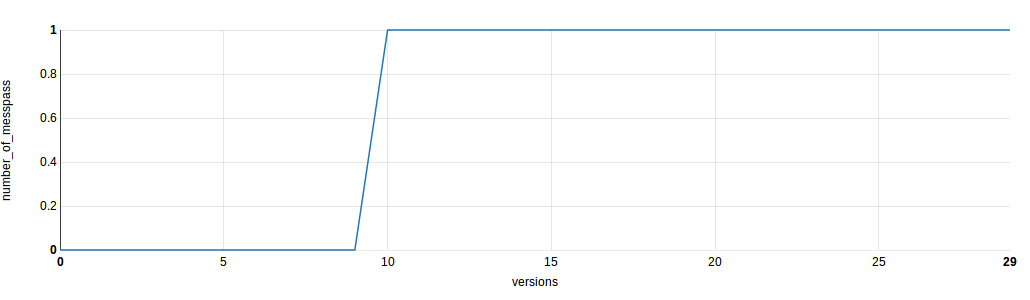
\includegraphics[height=45mm]{figures/chat.png}
	\caption{The number of message passing for module websocket\_handler.erl.}
	\label{fig:chat}
\end{figure}

As shown in Figure \ref{fig:chat5} there was increase in the length of the longest line of code in 9th version. 
\begin{figure}[h]
	\centering
	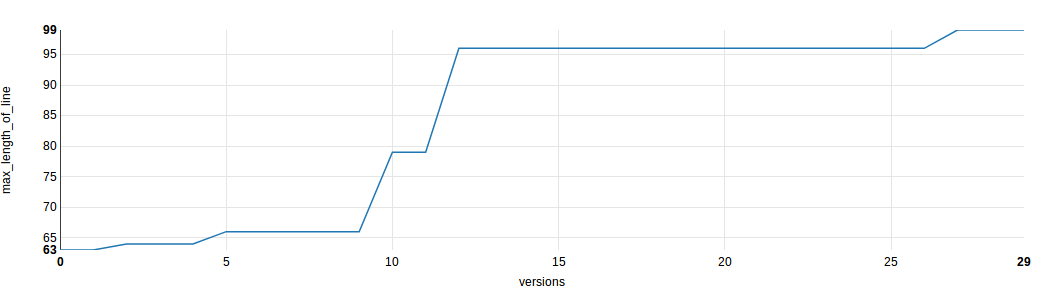
\includegraphics[height=45mm]{figures/chat5.png}
	\caption{Max length of line for module websocket\_handler.erl.}
	\label{fig:chat5}
\end{figure}

McCabe’s cyclomatic complexity metric measurement guarantees that developers are sensitive to the fact that programs with high McCabe numbers, for example, more than 10 are likely to be hard for understanding and accordingly have a higher probability of defects containing within the code base. The tested module has the cyclomatic complexity number which increased to 30 in the last versions as shown in Figure \ref{fig:mcCabe}.

\begin{figure}[h]
	\centering
	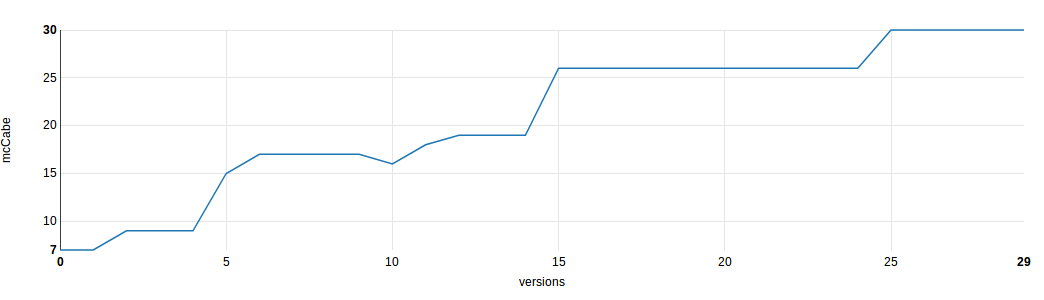
\includegraphics[height=45mm]{figures/mcCabe.png}
	\caption{
	McCabe cyclomatic complexity metric for module websocket\_handler.erl.}
	\label{fig:mcCabe}
\end{figure}

In Figure \ref{fig:chat2} shows that developer used otp library functions but after 9th version reconsidered to use them.

\begin{figure}[h]
	\centering
	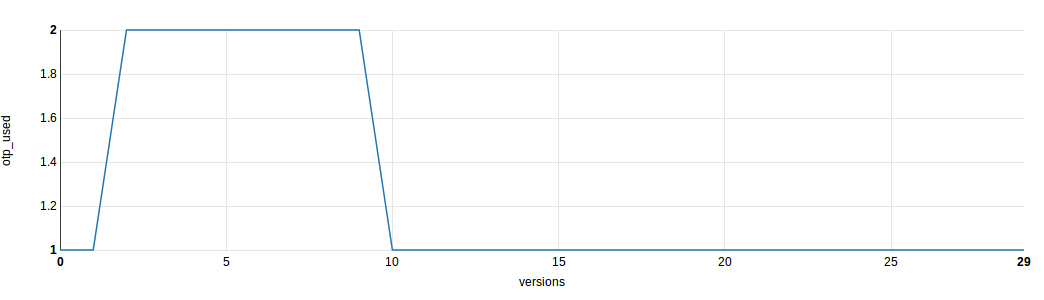
\includegraphics[height=45mm]{figures/chat2.png}
	\caption{Otp used for websocket\_handler.erl.}
	\label{fig:chat2}
\end{figure}

The developed framework allows measuring and visualizing metrics for a module and also for each function in the module. For example, in this module developer use message passing from the 9th version as we mentioned above. The Figure \ref{fig:chat3} shows that there was discovered function in which the author actively used message passing.

\begin{figure}[h]
	\centering
	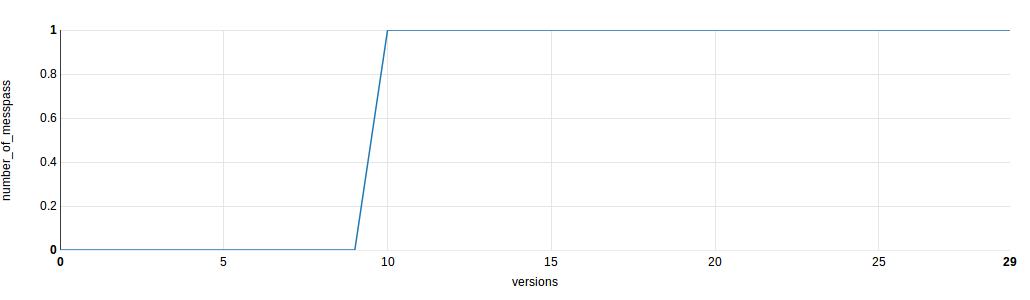
\includegraphics[height=45mm]{figures/chat3.png}
	\caption{Number of message passing for function websocket\_handle/3.}
	\label{fig:chat3}
\end{figure}

Visualizing of metrics helps to find which functions have been changed, added or deleted. As shown in the Figure \ref{fig:chat3} the developer slightly changed the function \textbf{terminate/3} by adding two lines of code in the 9th version.

\begin{figure}[h]
	\centering
	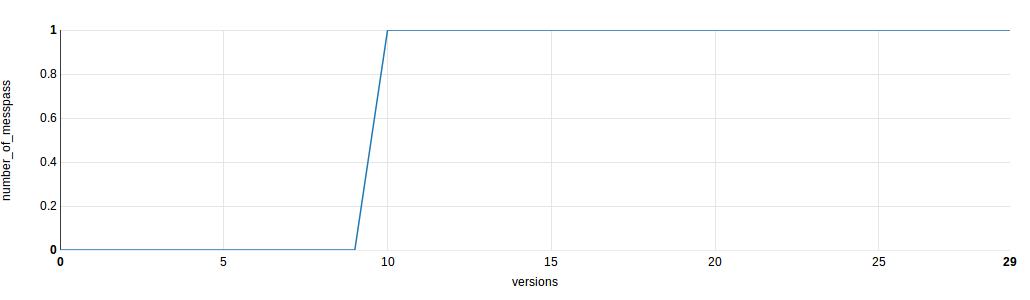
\includegraphics[height=45mm]{figures/chat3.png}
	\caption{
		Number of message passing for function websocket\_handle/3.}
	\label{fig:chat3}
\end{figure}
 
To summarize findings we can assume that most of these changes were done in the 9th version.

%%______________________________________________________

\section{prx}

This project is an Erlang library for Unix process management and system programming tasks. Code from all project is divided into 4 modules. 

The project provides:

\begin{itemize}
	\item Reliable operating system process management by mapping Erlang processes to a hierarchy of system processes.
	\item Beam-friendly interface for system calls and other POSIX operation.
	\item Operations for processes isolation like jails and containers.
	\item An interface for separation operations with privileges for processes restriction.
\end{itemize}


The link to the repository is \url{https://github.com/msantos/prx}. This project has 201 commits. 

For this project, we tested the module \textbf{prx.erl}. 

As in previous two experiments, at the beginning, we started to measure the \textbf{LOC} metric. This metric helps us to see the changes all of the project from over time. This result is shown in Figure \ref{fig:line_of_code_prx}.

\begin{figure}[h]
	\centering
	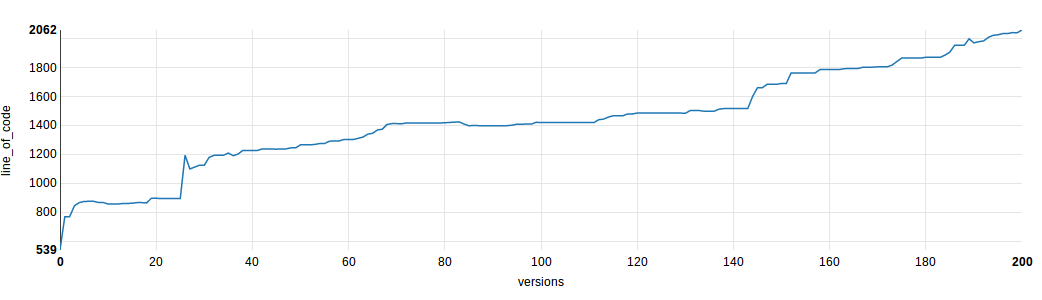
\includegraphics[height=45mm]{figures/line_of_code_prx.png}
	\caption{Effective Line of code for module prx.erl.}
	\label{fig:line_of_code_prx}
\end{figure}

Another important metric is \textbf{cohesion} metric. Modules with large cohesion number is preferable because high cohesion is associated with many desirable attributes of software such as robustness, reusability, reliability, and understandability. Otherwise, low cohesion is associated with undesirable attributes, for example, being difficult to reuse, maintain, test, or even understand. The Figure \ref{fig:cohesion_prx} and shows the decreasing of the calculated metric. 

\begin{figure}[h]
	\centering
	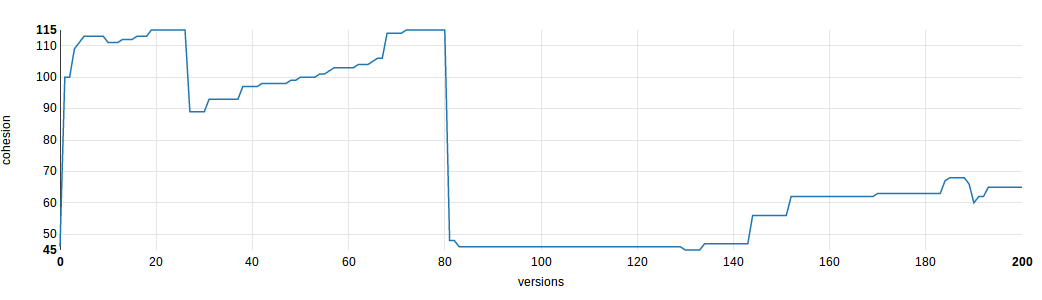
\includegraphics[height=45mm]{figures/cohesion_prx.png}
	\caption{The cohesion of the module prx.erl.}
	\label{fig:cohesion_prx}
\end{figure}

When developer started to use otp library in this project in 80th version, as we can see in Figure \ref{fig:otp_prx}, the McCabe cyclomatic complexity metric was rapidly increased in Figure \ref{fig:McCabe}. If complexity is increasing dramatically between versions, it is an indication of logic 
being added. 

\begin{figure}[h]
	\centering
	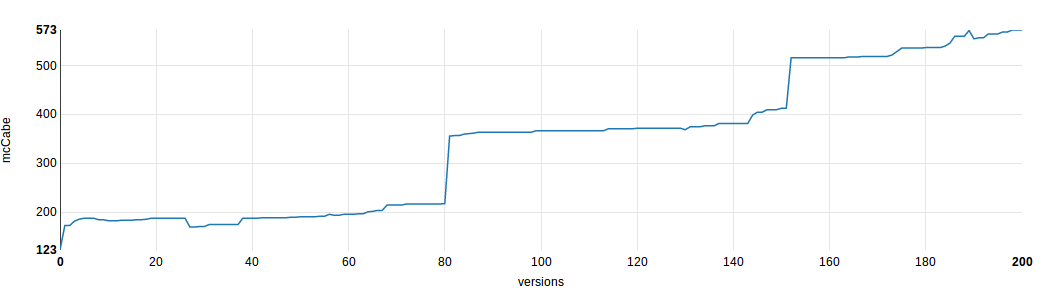
\includegraphics[height=45mm]{figures/mccabe.png}
	\caption{McCabe for the module prx.erl.}
	\label{fig:McCabe}
\end{figure}

When we are comparing results of cohesion and McCabe cyclomatic complexity metrics, we can conclude that low cohesion increases complexity, thereby increasing the likelihood of errors during the development process.

\begin{figure}[h]
	\centering
	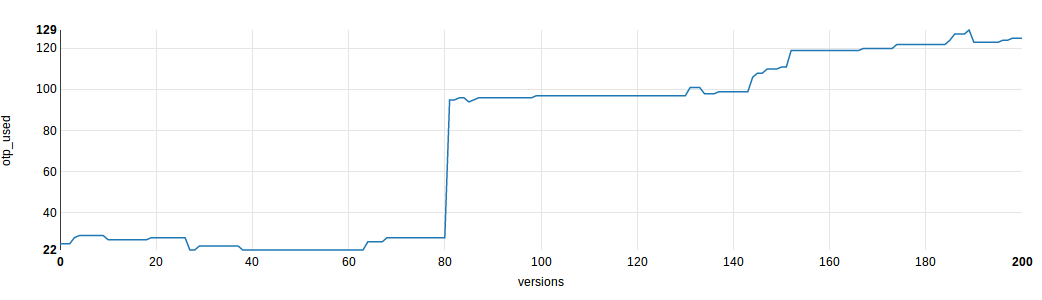
\includegraphics[height=45mm]{figures/otp_prx.png}
	\caption{OTP used for the module prx.erl.}
	\label{fig:otp_prx}
\end{figure}

Apart from analyzing the changes of the module we also can observe the changes of functions. The Figure \ref{fig:find/2} shows that the function \textbf{find/2} was used only in one version and later was renamed or deleted.

\begin{figure}[h]
	\centering
	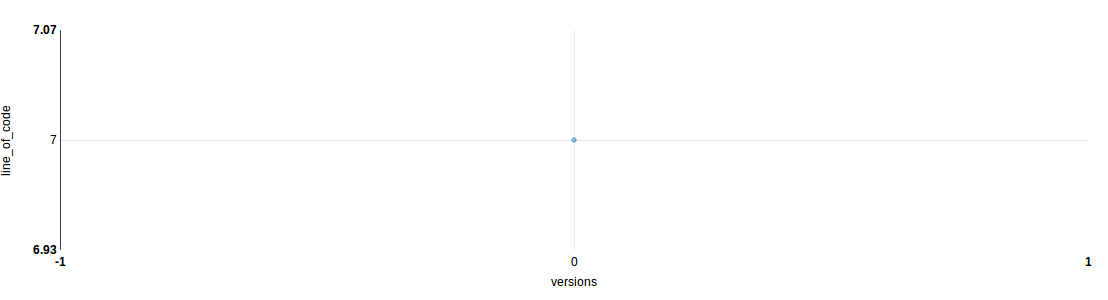
\includegraphics[height=45mm]{figures/find2.png}
	\caption{Effective Line of code for function find/2.}
	\label{fig:find/2}
\end{figure}

One of the features of functional programming languages is the presence of tail recursion. It is a special form of recursion where the last operation of a function is a recursive call ~\cite{tail}.
The metric \textbf{is\_tail\_recursive} returns with 1, if the given function is tail recursive; with 0, if it is recursive, but not tail recursive and -1 if it is not a recursive function. As shown in Figure \ref{fig:tail1} we can see that developer got rid of this function from 37th version until 40th version.

\begin{figure}[h]
	\centering
	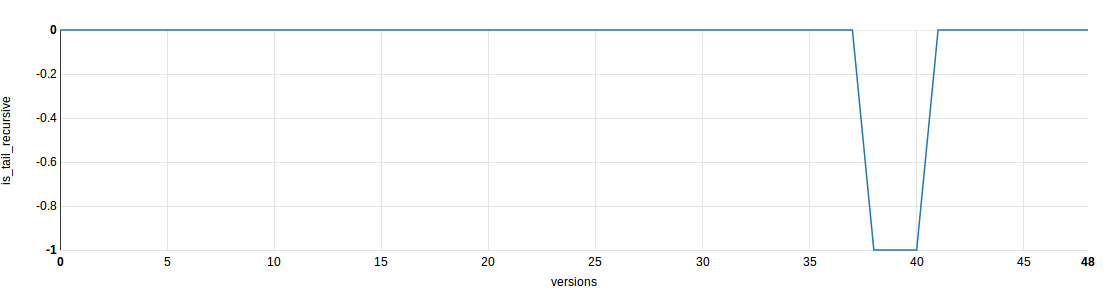
\includegraphics[height=45mm]{figures/filter2.png}
	\caption{Is tail recursive metric for function filter/2.}
	\label{fig:tail1}
\end{figure}

Also we can calculate how many times a function calls itself by using \textbf{branches\_of\_recursion} metric for all module. The Figure \ref{fig:br} illustrates that there were created more recursive functions after 140th version.

\begin{figure}[h]
	\centering
	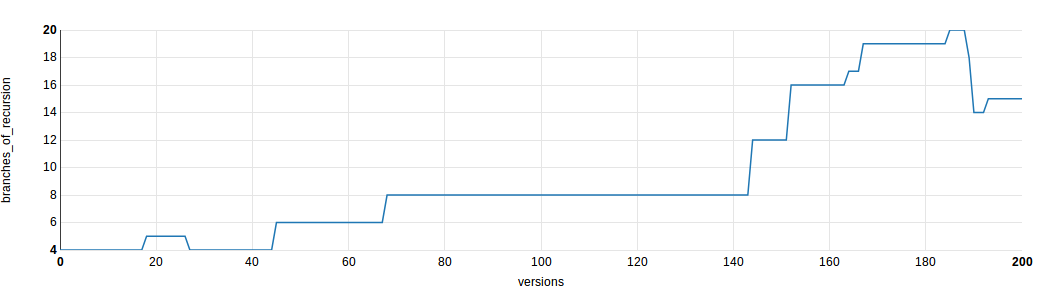
\includegraphics[height=45mm]{figures/br.png}
	\caption{Branches of recursion for module prx.erl.} 
	\label{fig:br}
\end{figure}

In RefactorErl there is a \textbf{function\_sum} metric which can be calculated using these metrics together: \textbf{line\_of\_code}, \textbf{char\_of\_code}, \textbf{number\_of\_funclauses}, \textbf{branches\_of\_recursion},
\textbf{mcCabe}, \textbf{calls\_for\_function}, \textbf{calls\_from\_function}, \textbf{fun\_return\_points}, \textbf{number\_of\_messpass}. Metrics \textbf{calls\_for\_function} and \textbf{calls\_from\_function} available only for functions. We can notice the dependency of \textbf{function\_sum} (Figure \ref{fig:function_sum_task4}) on two metrics changes: number of lines of code (Figure \ref{fig:task4}) and calls from the function (Figure \ref{fig:calls_from_function_task4}).

\begin{figure}[h]
	\centering
	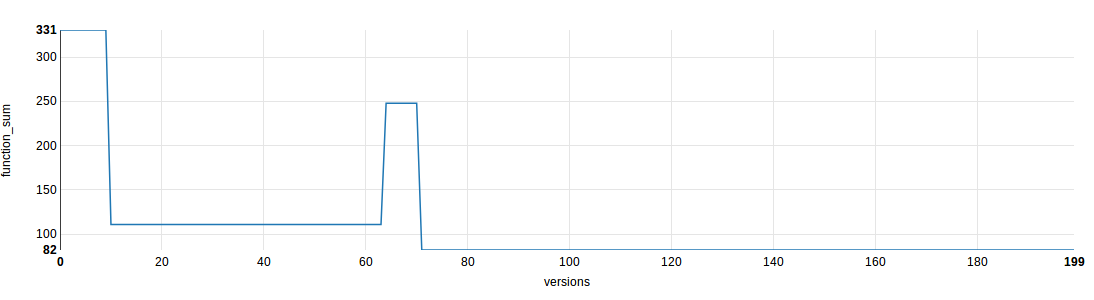
\includegraphics[height=45mm]{figures/function_sum_task4.png}
	\caption{Function sum function task/4.} 
	\label{fig:function_sum_task4}
\end{figure}

\begin{figure}[h]
	\centering
	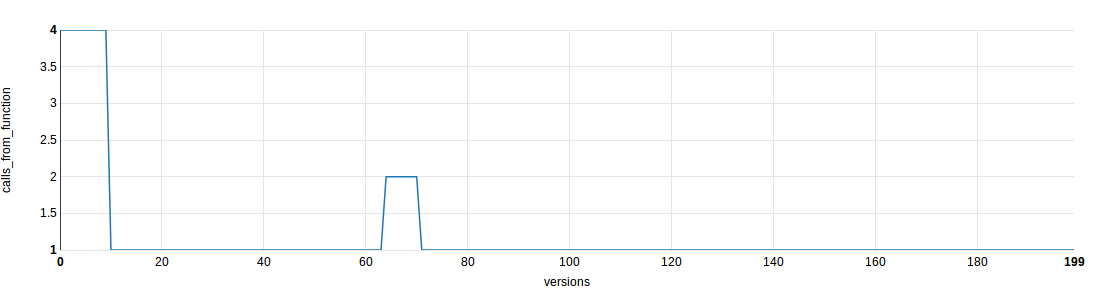
\includegraphics[height=45mm]{figures/calls_from_function_task4.png}
	\caption{Calls from the function for function task/4.} 
	\label{fig:calls_from_function_task4}
\end{figure}

\begin{figure}[h]
	\centering
	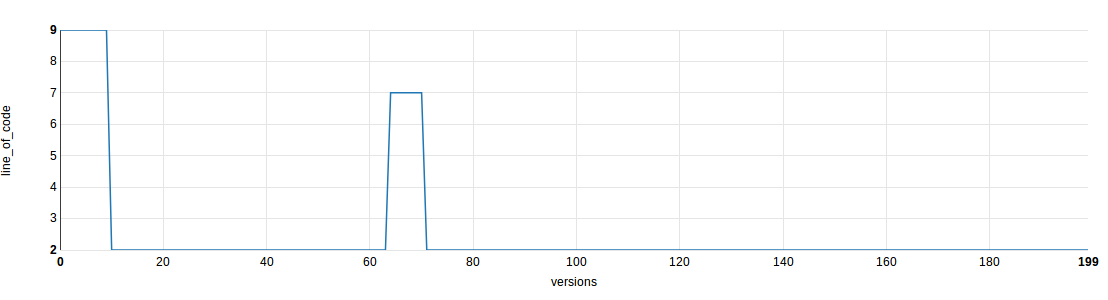
\includegraphics[height=45mm]{figures/task4.png}
	\caption{Effective Line of code for function task/4.} 
	\label{fig:task4}
\end{figure}